%%%%%%%%%%%%%%%%%%%%%%%%%%%%%%%%%%%%%%%%%%%%%%%%%%%%%%%%%%%%%%%%%%%
%                                                                 %
%                            APPENDICES                           %
%                                                                 %
%%%%%%%%%%%%%%%%%%%%%%%%%%%%%%%%%%%%%%%%%%%%%%%%%%%%%%%%%%%%%%%%%%%
 
\appendix    % This command is used only once!
%\addcontentsline{toc}{chapter}{APPENDICES}             %toc entry  or:
\addtocontents{toc}{\parindent0pt\vskip12pt APPENDICES} %toc entry, no page #

\chapter{Ontologies}
\section{PROV-PUB-O/S serialized in Turtle (TTL)}
\lstinputlisting{model/prov-pub-s.ls}
\section{PROV-PUB-O/S to DoCO bridging ontology}
\lstinputlisting{model/prov-pub-s-doco.ls}
\section{PROV-PUB-O/S to BIBO bridging ontology}
\lstinputlisting{model/prov-pub-s-bibo.ls}
\section{PROV-PUB-O/S to BibTeX bridging ontology}
\lstinputlisting{model/prov-pub-s-bibtex.ls}
\section{PROV-PUB-O/S usage examples}
\lstinputlisting{model/prov-pub-s-examples.ls}
\section{PROV-PUB-O/P serialized in Turtle (TTL)}
\lstinputlisting{model/prov-pub-p.ls}
\section{PROV-PUB-O/P usage examples}
\lstinputlisting{model/prov-pub-p-examples.ls}

\chapter{Case study details of the 5 figures and 3 tables in Chapter 4 of NCA 2014 report}
The case study is performed on Chapter 4, ``Energy supply and use'' of the National Climate Assessment Report 2014.

Chapter URI is \url{http://data.globalchange.gov/report/nca3/chapter/energy-supply-and-use}
Turtle file is \url{http://data.globalchange.gov/report/nca3/chapter/energy-supply-and-use.ttl}
This URL pattern applies for all the URIs below.

\textbf{Figure 4.1} is ``Paths of Hurricanes Katrina and Rita Relative to Oil and Gas Production Facilities''. The
figure URI is \url{http://data.globalchange.gov/report/nca3/chapter/energy-supply-and-use/figure/paths-of-hurricanes-katrina-and-rita-relative-to-oil-and-gas-production-facilities}.
This figure was derived from \url{http://data.globalchange.gov/report/gao-06-420t} --- ``Natural Gas: Factors Affecting Prices and Potential Impacts on Consumers (GAO-06-420T)'', the 
PDF file of this ``GAO-06-420T'' report is available at \url{http://www.gao.gov/assets/120/112796.pdf}.
Actually Figure 4.1 of NCA 2014 is almost the same as Figure 3 of the ``GAO-06-420T'' report, which has a note reads ``Source: GAO analysis of data provided by the National Weather Service and the Minerals Management Service.''
Only legends are found changed.

\textbf{Figure 4.2} is ``Increase in Cooling Demand and Decrease in Heating Demand''. The
percent differences are compared to the average for 1970-2000
Figure URI is \url{http://data.globalchange.gov/report/nca3/chapter/energy-supply-and-use/figure/increase-in-cooling-demand-and-decrease-in-heating-demand}
This figure was derived from \url{http://data.globalchange.gov/report/aeo2008} --- ``Annual Energy Outlook 2008 With Projections to 2030'', available at \url{http://www.eia.gov/oiaf/aeo/pdf/0383(2008).pdf}, but no clue relevant to this figure is found in this report.
The figure has an image \url{http://data.globalchange.gov/image/e7bdf318-1e1f-4c85-821f-907a55ff0ede}, which was derived from \url{http://data.globalchange.gov/dataset/nca3-heating-cooling-degree-day-data-r1}, which has a landing page at \url{http://www.ncdc.noaa.gov/oa/documentlibrary/hcs/hcs.html}. Footnote 16 of the chapter in NCA 2014 also says that data come from \url{http://www.ncdc.noaa.gov/oa/documentlibrary/hcs/hcs.html}
Raw data could be obtained by filling out the form at \url{http://www7.ncdc.noaa.gov/CDO/CDODivisionalSelect.jsp#} put for period 1970.1---2010.12.
This service is found by following a link at the hcs.html page: ``Item 14 on the NCDC Quick Links page'', and then click the ``Climate Indices'' hyperlink.
Temporary link to the raw data file was \url{http://www1.ncdc.noaa.gov/pub/orders/CDODiv8103636830652.txt}
Space separated raw data file can be found at  \url{http://www1.ncdc.noaa.gov/pub/orders/CDODiv2177686828992.txt}
This file became inaccessible after some time, so if we want to download the data again, we need to resubmit the request instead of re-accessing the temporary link to the raw data file.
A Jupyter Notebook --- nca3chapter4figure2no-output.ipynb --- was created which almost reproduced the result figure --- Figure 4.2.
Code of the Jupyter Notebook is shown in Figure~\ref{fig:nca3code} and the reproduced figure is shown in Figure~\ref{fig:nca3image}.
\begin{figure}
	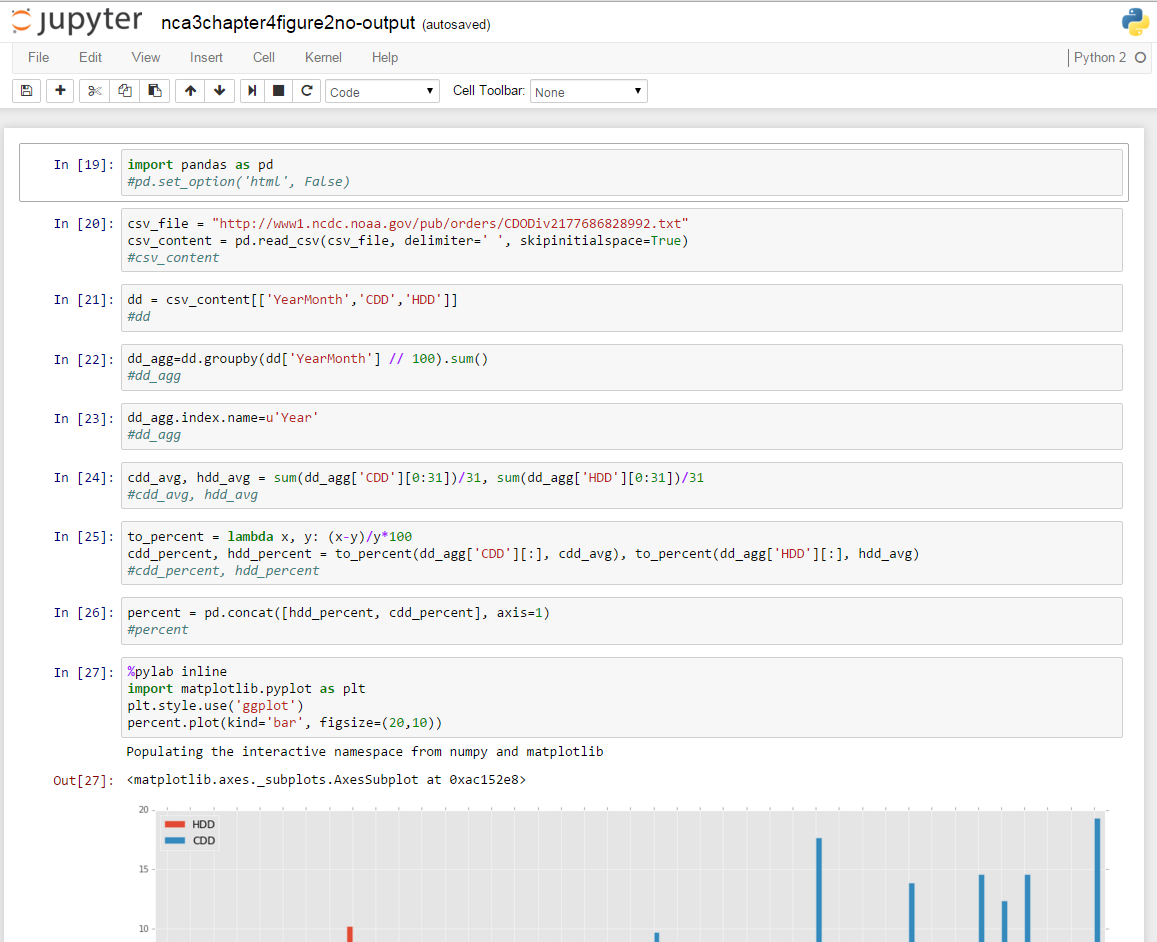
\includegraphics[width=\textwidth]{nca3code.png}
	\caption{Code reproducing Figure 4.2 of NCA 2014}
	\label{fig:nca3code}
\end{figure}
\begin{figure}
	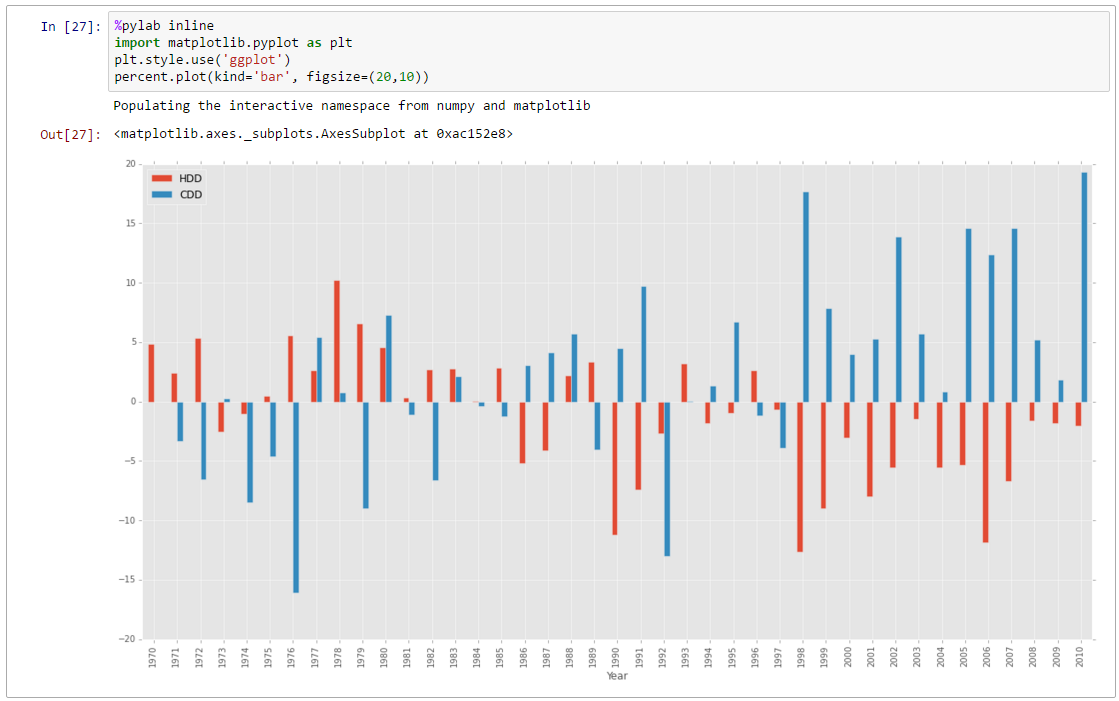
\includegraphics[width=\textwidth]{nca3image.png}
	\caption{The reproduced figure similar to Figure 4.2 of NCA 2014}
	\label{fig:nca3image}
\end{figure}

The textual description given in the caption of the figure is as follows:
\begin{quotation}
The amount of energy needed to cool (or warm) buildings is proportional to cooling (or heating) degree days. The figure shows increases in population-weighted cooling degree days, which result in increased air conditioning use, and decreases in population-weighted heating degree days, meaning less energy required to heat buildings in winter, compared to the average for 1970-2000. Cooling degree days are defined as the number of degrees that a day's average temperature is above 65°F, while heating degree days are the number of degrees a day’s average temperature is below 65°F. As shown, the increase in cooling needs is greater than the decrease in heating needs (Data from NOAA NCDC 2012).

\end{quotation}

The http://data.globalchange.gov/activity/e7bdf318-nca3-heating-cooling- degree-day-data-r1-process activity generated the image of this figure, but the activity does not include a ``qualifiedAssociation/hadPlan'' field to describe the detailed process of image generation. Some other activities mentioned later have such a field of textual description of the result generation method.

\textbf{Figure 4.3} is ``Increasing Numbers of Cooling Degree Days''. Figure URI is \url{http://data.globalchange.gov/report/nca3/chapter/energy-supply-and-use/figure/cooling-degree-days}.

This figure cites the article titled ``U.S. Population Projections'', accessible at \url{http://www.census.gov/population/projections/}, the article is not directly related to the figure, but just an additional comment to the figure (population projections suggest continued shifts toward areas that require air conditioning in the summer).

This figure mentioned in its caption that the figure source is NOAA NCDC / CICS-NC, but we cannot find the related resources by searching with these keywords on the Web.

A2 and B1 are two scenarios defined in the IPCC (Intergovernmental Panel on Climate Change) Special Report on Emission Scenarios (SRES)

The four images in this figure such as \url{http://data.globalchange.gov/image/f6db3545-873b-4c9e-b857-c3bb5671aea4}, ``Increasing Numbers of Cooling Degree Days: Higher Emissions (A2), 2021-2050'', are all derived from the dataset \url{http://data.globalchange.gov/image/nca3-cmip3-downscaled-r201304}. The dataset has a landing page at \url{http://cida.usgs.gov/thredds/catalog.html}. Its title is ``Eighth degree-CONUS Daily Downscaled Climate Projections''. A report on this dataset can be found at \url{http://cida.usgs.gov/thredds/fileServer/dcp/files/Hayhoe_USGS_downscaled_database_final_report.pdf}, but the report is not helpful to finding the provenance.

Following a link at \url{http://cida.usgs.gov/thredds/catalog.html}, at \url{http://cida.usgs.gov/thredds/catalog.html?dataset=cida.usgs.gov/thredds/dcp/conus_t}, a dataset called ``1/8 degree-CONUS Daily Downscaled Climate Projections Minimum and Maximum Temperature'' is found. It has a lot of variables together: ccsm, cgcm3-t47, cgcm3-t63, cnrm, csiro, echam5, echo, gfdl, giss\_aom, hadcm3, hadgem, miroc\_hi, mri\_cgcm2, and pcm. 

We can use the netCDF subset service at \url{http://cida.usgs.gov/thredds/ncss/dcp/conus_t/dataset.html} to download a subset of the dataset as a netCDF file. One year of ccsm a2 tmax data are 286MB in size.

NCSS Request URL is of the form \url{http://cida.usgs.gov/thredds/ncss/dcp/conus_t?var=ccsm-a2-tmax-NAm-grid&disableLLSubset=on&disableProjSubset=on&horizStride=1&time_start=1960-01-01T00%3A00%3A00Z&time_end=2099-12-31T00%3A00%3A00Z&timeStride=1}

Following a link at \url{http://cida.usgs.gov/thredds/catalog.html?dataset=cida.usgs.gov/thredds/dcp/conus_t}, we went to \url{http://cida.usgs.gov/thredds/uddc/dcp/conus_t?catalog=http%3A%2F%2Fcida.usgs.gov%2Fthredds%2Fcatalog.html&dataset=cida.usgs.gov%2Fthredds%2Fdcp%2Fconus_t}. 
	The page has title: Eighth degree-CONUS Daily Downscaled Climate Projections by Katharine Hayhoe, which is an exact match with the dataset description in the data.globalchange.gov provenance graph, but it is just a quality assessment of the data set in terms of attribute convention. We cannot find the raw data.

The prov:hadPlan field of the prov:qualifiedAssociation field of the activity \url{http://data.globalchange.gov/activity/f6db3545-nca3-cmip3-downscaled-r201304-process} describes the algorithm:
\begin{enumerate}
\item For each model at each grid point, the number of cooling degree days under the higher emissions scenario (A2) was calculated for two periods: 1971--2000 and 2021--2050. According to the figure 4.2 caption, ``Cooling degree days are defined as the number of degrees that a day's average temperature is above 65$^{\circ}$F'', yet the dataset has no ``average temperature'' variable, but only max and min temperature values. How the number of cooling degree days is calculated remains unclear.
\item At each grid point, the number of cooling degree days was computed for both time periods by averaging the following models:
\begin{itemize}
\item cgcm3\_t47
\item cgcm3\_t63
\item cnrm
\item echam5
\item echo
\item gfdl\_2.1
\item hadcm3
\item pcm
\end{itemize}

\item At each grid point, the difference in the number of cooling degree days was calculated for 2021--2050 minus 1971--2000.
\item Data were plotted for all grid points.
\end{enumerate}

The image \url{http://data.globalchange.gov/image/f6db3545-873b-4c9e-b857-c3bb5671aea4}, ``Increasing Numbers of Cooling Degree Days: Higher Emissions (A2), 2021--2050'', was generated by the above process.

\textbf{Figure~4.4} is ``Projected Changes in Seasonal Precipitation''
Figure URI is \url{http://data.globalchange.gov/report/nca3/chapter/energy-supply-and-use/figure/projected-changes-in-seasonal-precipitation}.
Same as Figure~4.3, this figure also cites NOAA NCDC / CICS-NC.
The upper-left image of this figure --- ``Projected Changes in Seasonal Precipitation - Winter'' (URI is \url{http://data.globalchange.gov/image/5ae3d8d8-64d1-4dab-a08a-4ec46a58e3da}) --- was derived from World Climate Research Programme's (WCRP's) Coupled Model Intercomparison Project phase 3 (CMIP3) multi-model dataset, the identifier of the dataset is \url{http://data.globalchange.gov/dataset/nca3-cmip3-r201205}, and the landing page is \url{http://www-pcmdi.llnl.gov/ipcc/about_ipcc.php}. Downloading the data requires registration and approval from the administrator. It took 4 days to finish my registration process.
The activity with the URI \url{http://data.globalchange.gov/activity/5ae3d8d8-nca3-cmip3-r201205-process} has the description of the process that generated the image.
All the four images in this figure are described in the same manner.
The prov:hadPlan field of the prov:qualifiedAssociation field for the process (hopefully how to use the data at \url{http://www-pcmdi.llnl.gov/ipcc/about_ipcc.php}) is:
\begin{enumerate}
\item For each model at each grid point, the mean winter precipitation under the higher emissions scenario (A2) was calculated.
\item For each model, these data were re-gridded to a common grid.
\item For each model at each grid point, the mean winter precipitation under the higher emissions scenario (A2) was calculated for two periods: 1970--1999 and 2041--2070.
\item At each grid point, the mean winter precipitation for the two periods was computed by averaging the following models:
CCSM3, CGCM3.1 (T47), CNRM-CM3, CSIRO-Mk3.0, ECHAM5/MPI-OM, ECHO-G, GFDL-CM2.0, GFDL-CM2.1, INM-CM3.0, IPSL-CM4, MIROC3.2 (medres), MRI-CGCM2.3.2, PCM, UKMO-HadCM3, and UKMO-HadGEM1
\item At each grid point, the difference in projected winter precipitation was calculated for 2041-2070 minus 1970-1999.
\item Data were plotted for grid points in the United States with hatching/white-out applied as follows:
If less than 50\% of the models show a statistically significant change, then those grid points are whited out. If more than 50\% of the models show a statistically significant change, but less than 67\% of the models agree on the sign of the change, then those grid points are shaded. If more than 50\% of the models show a statistically significant change, and more than 67\% of the models agree on the sign of the change, then shading is overlaid with hatching for those grid points.
\end{enumerate} 
How ``mean winter precipitation'' is calculated at the fourth step of the plan is unclear. Because only daily, weekly, monthly and yearly means are given in the data files for the following models.

Following a link at \url{http://www-pcmdi.llnl.gov/ipcc/about_ipcc.php}, we get to the page \url{http://www-pcmdi.llnl.gov/ipcc/orientation.php}, which has a link to \url{http://www-pcmdi.llnl.gov/ipcc/data_status_tables.htm}, we can see SRESA2 is among the column titles, and CCSM3, CGCM3.1 (T47), CNRM-CM3, CSIRO-Mk3.0, ECHAM5/MPI-OM, ECHO-G, GFDL-CM2.0, GFDL-CM2.1, INM-CM3.0, IPSL-CM4, MIROC3.2 (medres), MRI-CGCM2.3.2, PCM, UKMO-HadCM3, and UKMO-HadGEM1 are all there, but others in the table are not included by the process plan.

Following another link at \url{http://www-pcmdi.llnl.gov/ipcc/about_ipcc.php}, we get to \url{https://esg.llnl.gov:8443/about/ipccTables.do}, where we know that ``pr'' is for Precipitation.
Yet another link at \url{http://www-pcmdi.llnl.gov/ipcc/about_ipcc.php}  to \url{https://esg.llnl.gov:8443/about/search.do} instructs users how to search the datasets.
At \url{https://esg.llnl.gov:8443/data/advancedSearchPage.do}, we can search for SRES A2 experiment, CGCM3.1 T47 and get Run1--5 monthly data.
The site is having issues with data browsing and downloading, we are advised to go to \url{ftp://ftp-esg.ucllnl.org} instead, where we can find a sresa2 directory, with 4 empty files. There is a FTP sitemap at \url{https://esg.llnl.gov:8443/about/ftp.do}, which points us to sresa2, the empty directory again.

\textbf{Figure~4.5} is ``California Power Plants Potentially at Risk from Sea Level Rise''.
Its URI is \url{http://data.globalchange.gov/report/nca3/chapter/energy-supply-and-use/figure/california-power-plants-potentially-at-risk-from-sea-level-rise}
It is derived from ``Estimating Risk to California Energy Infrastructure from Projected Climate Change'', and its
URI is \url{http://data.globalchange.gov/report/osti-1026811}. 
The report could be found at \url{http://www.energy.ca.gov/2012publications/CEC-500-2012-057/CEC-500-2012-057.pdf}, but there is no direct link to this paper source in the provenance graph.
Figure~19 of the report --- ``Power Plants Potentially at Risk to a 100-year Flood with a 1.4 m Sea Level Rise'' --- is reused as Figure~4.5 in this chapter, but this fact is not specified and this is a 88-page report and it is not easy to find the figure being reused.

\textbf{Table~4.1} is ``Changing Energy Use for Heating and Cooling Will Vary by Region''. Its 
URI is \url{http://data.globalchange.gov/report/nca3/chapter/energy-supply-and-use/table/energy-regional-impacts}.
The table cites \url{http://data.globalchange.gov/report/noaa-techreport-nesdis-142-[1-6]} each of these citations' gcis:hasURL property value points to the PDF file of the report.
The caption of the table says ``Table information is adapted from multi-model means from 8 NARCCAP regional climate simulations for the higher emissions scenario (A2) considered in this report and is weighted by population.'' in reference 20 of the chapter, the 6 reports this table is based on are listed.
Questions need clarifications are:
\begin{itemize}
\item How these days are weighted by population? 
\item What kind of adaptation has been done? 
\item Is the adaptation just the ``population weighting'' calculation?
\end{itemize}
In NOAA Techreport NESDIS 142-1 about the Northeast area, Figures 25 and 26 are about 2041--2070 mean minus 1980--2000 mean, which does not fit the time frame of Table~4.1.
Table 5 of each report in NOAA Techreport DESDIS 142-[1--6] have relevant data with Table~4.1 but different values.
For example, Table~4.1 says for Northeast +10 days extreme hot days (>95F), but Table~5 of 142-1 says +8 days for NARCCAP Mean, and Table~4.1 says +77\% increase in CDDs per year (2041--2070 above 1971--2000), but Table~5 says +99\%. Details of these differences are listed as follows:

Northeast:

\begin{tabular}{|l|p{0.15\textwidth}|p{0.15\textwidth}|p{0.1\textwidth}|p{0.15\textwidth}|}
	\hline
Source & Additional >95F days & \% Increase in CDDs & Fewer <10F days & \% Decrease in HDDs \\ 
\hline
Table~4.1 in NCA3	& +10 days & +77\% & -12 days & -17\% \\ 
\hline
Table~5 in 142-1	& +8 days & +99\% & -17 days & -16\% \\
\hline
\end{tabular}

\mbox{}

Southeast:

\begin{tabular}{|l|p{0.15\textwidth}|p{0.15\textwidth}|p{0.1\textwidth}|p{0.15\textwidth}|}
	\hline
	Source & Additional >95F days & \% Increase in CDDs & Fewer <10F days & \% Decrease in HDDs \\ 
	\hline
Table~4.1 in NCA3 & +23 days & +43\% & -2 days & -19\% \\
\hline
Table~5 in 142-2 & +27 days & +49\% & -2 days & -19\% \\
\hline
\end{tabular}

\mbox{}

Midwest:

\begin{tabular}{|l|p{0.15\textwidth}|p{0.15\textwidth}|p{0.1\textwidth}|p{0.15\textwidth}|}
	\hline
	Source & Additional >95F days & \% Increase in CDDs & Fewer <10F days & \% Decrease in HDDs \\ 
	\hline
	Table~4.1 in NCA3 & +14 days & +64\% & -14 days & -15\% \\
	\hline
Table~5 in 142-3 & +15 days & +66\% & -16 days & -16\% \\
\hline
\end{tabular}

\mbox{}

Great Plains:

\begin{tabular}{|l|p{0.15\textwidth}|p{0.15\textwidth}|p{0.1\textwidth}|p{0.15\textwidth}|}
	\hline
	Source & Additional >95F days & \% Increase in CDDs & Fewer <10F days & \% Decrease in HDDs \\ 
	\hline
	Table~4.1 in NCA3 & +22 days & +37\% & -4 days & -18\% \\
	\hline
	Table~5 in 142-4 & +18 days & +48\% & -12 days & -16\% \\
	\hline
\end{tabular}

\mbox{}

Southwest:

\begin{tabular}{|l|p{0.15\textwidth}|p{0.15\textwidth}|p{0.1\textwidth}|p{0.15\textwidth}|}
	\hline
	Source & Additional >95F days & \% Increase in CDDs & Fewer <10F days & \% Decrease in HDDs \\ 
	\hline
	Table~4.1 in NCA3 & +20 days & +44\% & -3 days & -20\% \\
	\hline
	Table~5 in 142-5 & +20 days & +64\% & -11 days & -18\% \\
	\hline
\end{tabular}

\mbox{}

Northwest:

\begin{tabular}{|l|p{0.15\textwidth}|p{0.15\textwidth}|p{0.1\textwidth}|p{0.15\textwidth}|}
	\hline
	Source & Additional >95F days & \% Increase in CDDs & Fewer <10F days & \% Decrease in HDDs \\ 
	\hline
	Table~4.1 in NCA3 & +5 days & +89\% & -7 days & -15\% \\
	\hline
	Table~5 in 142-6 & +5 days & +105\% & -15 days & -15\% \\
	\hline
\end{tabular}

\mbox{}

\textbf{Table~4.2} is ``Possible Climate Resilience and Adaptation Actions in Energy Sector''. It has URI: \url{http://data.globalchange.gov/report/nca3/chapter/energy-supply-and-use/table/energy-adaptation}.
The table cites \url{http://data.globalchange.gov/report/ornl-climchinfrastructure-2012}, which has URL \url{http://www.esd.ornl.gov/eess/Infrastructure.pdf}.
It is a table listing items and their attributes, instead of the result of changes of data.

\textbf{Table~4.3} is ``Energy Supply: Summary of National and Regional Impacts, Challenges and Opportunities''. It has
URI: \url{http://data.globalchange.gov/report/nca3/chapter/energy-supply-and-use/table/energy-supply-national-regional}.
This table cites \url{http://data.globalchange.gov/report/ornl-climchinfrastructure-2012}, and \url{http://data.globalchange.gov/report/ccsp-sap-2_1a-2007}, which has URL \url{http://downloads.globalchange.gov/sap/sap2-1a/sap2-1a-final-all.pdf}.
Notes for column ``mean annual temperature'' and ``summer precipitation'': CMIP3 15 GCM Models: 2070--2099 Combined Interquartile Ranges of SRES B1 and A2 (versus 1971--2000), incorporating uncertainties from both differences in model climate sensitivity and differences between B1 and A2 in emissions trajectories.

Notes for ``sea level rise (2100)'': Range of sea level rise for 2100 is the Low Intermediate to High Intermediate Scenario from ``Sea Level Change Scenarios for the U.S. National Climate Assessment.'' Range is similar to the 1 to 4 feet of sea level rise projected in Ch. 2: Our Changing Climate, Key Message 10. There will be regional variations in sea level rise, and this category of impacts does not apply for the Midwest region.

Notes for ``\#Days >90F (2055)'' has references \url{http://data.globalchange.gov/report/ornl-climchinfrastructure-2012} and \url{http://data.globalchange.gov/report/ccsp-sap-2_1a-2007}, how these numbers are obtained is not found yet.

\chapter{Prototype source code}
\section{provmagic.py}
\lstinputlisting[language=Python,breaklines=true]{scripts/prov/provmagic.py}
\section{operators.py}
\lstinputlisting[language=Python,breaklines=true]{scripts/prov/operators.py}
\section{dataloader.py}
\lstinputlisting[language=Python,breaklines=true]{scripts/prov/dataloader.py}
\section{datatransformer.py}
\lstinputlisting[language=Python,breaklines=true]{scripts/prov/datatransformer.py}
\section{datasaver.py}
\lstinputlisting[language=Python,breaklines=true]{scripts/prov/datasaver.py}
\section{dataplotter.py}
\lstinputlisting[language=Python,breaklines=true]{scripts/prov/dataplotter.py}

%This is how equations are numbered in an appendix:
%\begin{equation}
%x^2 + y^2 = z^2
%\end{equation} 
%This is a sentence to take up space and look like text.
%This is a sentence to take up space and look like text.
%This is a sentence to take up space and look like text.
% 
%This is a sentence to take up space and look like text.
%This is a sentence to take up space and look like text.
%This is a sentence to take up space and look like text.
%This is a sentence to take up space and look like text.
%This is a sentence to take up space and look like text. 

%\chapter{THIS IS ANOTHER APPENDIX} 
%This is a sentence to take up space and look like text.
%This is a sentence to take up space and look like text.
%This is a sentence to take up space and look like text.
%This is a sentence to take up space and look like text.
%This is a sentence to take up space and look like text.
%This is a sentence to take up space and look like text.
%This is a sentence to take up space and look like text.
%This is a sentence to take up space and look like text.
 
